\documentclass[article, 10pt, type=bsc, colorback, accentcolor=tud8b, parskip=half, bibliography=totocnumbered]{tudthesis}

\usepackage[utf8]{inputenc}
\usepackage{listings}
\usepackage{graphicx}
\usepackage[backend=biber, citestyle=numeric-comp, sorting=none]{biblatex}

\lstset{basicstyle=\ttfamily}

\addbibresource{references.bib}

\newcommand{\comment}[1]{}

\begin{document}

\thesistitle{EventScala}{A Type-Safe, Distributed and Quality-of-Service-oriented Approach to Event Processing}
\author{Lucas Konstantin Bärenfänger}
\referee{Prof. Dr. Guido Salvaneschi}{Pascal Weisenburger, M.Sc.}
\department{Fachbereich Informatik}
\group{Software Technology Group\newline Reactive Programming Technology}

\makethesistitle

\affidavit{Lucas Konstantin Bärenfänger}

\tableofcontents

\newpage

\section{Abstract}
\label{sec:abstract}

Many of today's software systems rely on event processing (EP) for analyzing and reacting to events in real-time, including business-critical applications.

However, current EP solutions suffer from shortcomings, of which the following three are subject of this thesis.
For one, EP queries are commonly expressed in the form of strings, allowing for no syntax and type checking at compile-time.
Furthermore, many solutions employ a non-distributed, i.e., centralized, approach.
Lastly, there appears to be no solution that enables queries to be annotated with quality of service (QoS) requirements.

The contribution of this thesis, the EventScala framework, sets out to explore ways to tackle these issues.
To this end, EventScala features a domain-specific language (DSL) for expressing queries in a type-safe, statically checked fashion.
Moreover, to achieve distributed execution, EventScala's execution engine runs queries by mapping their primitives and operators to concurrently executing nodes, which form a graph that resembles the structure of the given query.
Finally, in EventScala, the annotation of queries with QoS requirements is supported at both the language and the execution level.

EventScala is based on the Scala technology stack.
The DSL leverages the flexibility and extensibility of the Scala programming language.
The execution engine leverages the Akka toolkit's abstractions for concurrent programming.

\newpage

\section{Introduction}
\label{sec:introduction}

Event processing (EP) is now the ``paradigm of choice'' \cite{Hinze:2009:EAE:1619258.1619260} for building applications that analyze and react to events as they happen.
In the corporate world, it is used in a variety of applications, e.g., business process management \cite{Buchmann:2012:CEA:2413516.2413519}.
EP technology is also deeply embedded in the financial sector.

Nevertheless, current EP solutions still suffer from shortcomings, three of which are addressed in this thesis.
For one, many EP solutions, e.g., Esper \cite{esper}, receive queries in the form of strings, just like it is common in the field of relational databases.
As a consequence, syntactically malformed or ill-typed queries are not detected at compile-time, allowing for them to fail at run-time.
Furthermore, most if not all industry-grade EP solutions are non-distributed \cite{Schilling:2010:DHE:1827418.1827453}, i.e., centralized, solutions.
Therefore, they can neither leverage parallelism to meet efficiency demands nor do they cope with the distributed nature of event sources.
Lastly, while some research has been conducted on quality of service (QoS) in the EP domain (section \ref{sec:ep_distributed_execution}), there appears to be no solution enabling queries to be explicitly annotated with QoS requirements.
However---especially in the case of real-time applications that make decisions---whether or not a query's requirements have been met during its execution might be crucial for the value and/or correctness of its result.

This thesis presents a type-safe, distributed and QoS-oriented approach to EP.
As such, it explores ways to tackle the aforementioned issues.
Its contribution, the EventScala framework, features a domain-specific language (DSL) for expressing EP queries as well as an execution engine for running them.
The DSL enables to express queries in a type-safe manner, thus, serves as a static shield against malformed or ill-typed queries.
It also allows for QoS requirements to be defined over queries in a fine-grained fashion, i.e., they can be defined over a query or its arbitrarily deeply nested subqueries.
The execution engine enables queries to be run in a distributed fashion by mapping the primitives and operators of a given query to concurrently executing processing nodes, which form a graph that resembles the structure of said query.
Each processing node continuously monitors its performance and triggers user-defined action whenever a QoS requirement is not met.

EventScala is based on the technology stack of the Scala ecosystem.
Due to its flexible and extensible nature, the Scala programming language is known for its support for building DSLs.
Therefore, the DSL is embedded into Scala, leveraging some of the features that make Scala a great host language, e.g., infix operator syntax and implicit conversions.
The execution engine is built upon the abstractions provided by the Akka toolkit \cite{akka}.
Akka's approach to concurrency programming is based on the actor model \cite{Hewitt:1973:UMA:1624775.1624804}, aiming to eliminate many of the difficulties commonly associated with the subject.
Moreover, Akka appears to be especially suited for developing an EP solution, as it already embodies several of the characteristics common in the EP domain.

It can be stated that expressing queries using the DSL as opposed to SQL-like strings is a superior approach.
One reason for this is that statically checked queries are far less likely to fail at run-time.
Furthermore, running queries using the execution engine constitutes a way to benefit from the advantages of concurrent execution in the EP domain.
Finally, this thesis shows that the concept of queries being annotated with QoS requirements can be incorporated at the language as well as at the execution level.

The remainder of this thesis is structured as follows.
Related work is presented in section \ref{sec:state_of_the_art}.
The state of the art of EP in general is covered in section \ref{sec:event_processing}, its language-level integration is discussed in section \ref{sec:ep_language_integration}, and sections \ref{sec:ep_distributed_execution} and \ref{sec:ep_qos} deal with distributed EP as well as QoS in the context of EP, respectively.
Section \ref{sec:eventscala} presents the EventScala framework, with section \ref{sec:case_class_rep} introducing the underlying case class representation, section \ref{sec:dsl} covering the DSL, section \ref{sec:execution_engine} discussing the execution level and section \ref{sec:qos} outlining the QoS approach.
A simulation showcasing EventScala's capabilities is presented in section \ref{sec:simulation}.
This thesis is concluded in section \ref{sec:conclusion}. 

\newpage

\section{State of the Art}
\label{sec:state_of_the_art}

\subsection{Event Processing (EP)}
\label{sec:event_processing}

Event processing (EP) has, according to Hinze, Sachs and Buchmann \cite{Hinze:2009:EAE:1619258.1619260}, become the ``paradigm of choice in many monitoring and reactive applications'', with application scenarios including traffic monitoring, fraud detection, supply chain management and many more.
(Refer to their paper ``Event-based Applications and Enabling Technologies'' \cite{Hinze:2009:EAE:1619258.1619260} for an extensive list of use cases.)

This section introduces terminology as well as concepts common the EP field.
In the end, some noteworthy EP solutions as well as the respective publications are referenced.

Chandy and Schulte \cite{Chandy:2009:EPD:1594754} describe an event as ``something that happens''.
Hinze, Sachs and Buchmann \cite{Hinze:2009:EAE:1619258.1619260} introduce two more refined notions of events:
``change events'', e.g., an object changing its position, and ``status events'', e.g., a value yielded by a sensor.

After being observed and signaled, an event takes the form of an event instance, which corresponds to an event type.
An event instance is commonly represented as a tuple of values, with the type of each element of the tuple being defined by the associated event type.
For example, a temperature reading from a sensor ``X'' indicating 21 °C in temperature might be represented by the event instance \lstinline{("X", 21)} with the event type being \lstinline{(String, Int)}.
For the sake of simplicity, the remainder of this thesis will refer to event instances as events.

Analogous to expressions in programming languages, which are either primitive values, e.g., \lstinline{true} or \lstinline{42}, or made up of other expressions that are combined by operators and/or functions, e.g., \lstinline{true && isThisAGoodNumber(42)}, events may be primitive events or compositions/derivations of primitive and/or other composite/derived events.
According to the definitions by Hinze, Sachs and Buchmann \cite{Hinze:2009:EAE:1619258.1619260}, ``composite events'' are ``aggregations of events'', whereas ``derived events'' are ``caused by other events'' and typically are ``at a different level of abstraction''.
As an example of the latter, consider a series of failed login attempts might cause an intrusion event.

Etzion and Neblett \cite{Etzion:2010:EPA:1894960} define an ``event stream (or stream)'' as a ``set of associated events'' that is ``often'' ``temporally ordered''.
A stream solely consisting of events of the same type is called a ``homogeneous stream''---as opposed to ``heterogeneous''.

Operators are defined over streams---as opposed to individual events.
The \lstinline{or} operator, for example, represents the union of two streams, and places the events of both streams in one result stream.
The two streams the \lstinline{or} operator takes as operands can be viewed as its incoming streams, the result stream can be viewed as its outgoing stream.

Traditionally, two approaches to EP can be distinguished:

\begin{description}
\item[Stream processing (SP)]
SP typically features operators that resemble those of relational algebra, e.g., \lstinline{projection}, \lstinline{selection}, \lstinline{join}, etc.
SP queries are usually expressed in some SQL dialect and constitute so-called ``continuous queries''.
This term underlines an inversion of principles: In traditional database management systems (DBMSs), it is the data that is being persisted and not the queries. Continuous queries, however, are being persisted and run \emph{continuous}ly, while it is the data that can be thought of as flowing through.
\item[Complex event processing (CEP)]
CEP typically features operators that resemble those of boolean algebra, e.g., \lstinline{and}, \lstinline{or}, \lstinline{not}.
Operators such as \lstinline{sequence} and \lstinline{closure} are common, too. CEP queries are usually expressed using rule languages.
\end{description}

There is another significant difference between SP and CEP.
As said, SP operators resemble those of relational algebra.
Some relational operators (e.g., \lstinline{join}), however, are blocking operators, i.e., blocking in the sense that they are defined over finite sets of data and block execution until these are available in their entirety.
Streams, however, can be viewed as infinite sets of data.
As a consequence, in SP, the respective operators are not applied to streams directly.
Instead, they require their operand streams to be annotated with so-called windows, which are typically expressed ``in terms of time or number of tuples [i.e., events]'' \cite{Chakravarthy:2009:SDP:1550717}.
At any point in time, a window only contains a finite number of the events of the respective stream.
So-called consumption modes are the counterpart of windows in CEP.
They are explained best through an example.
The CEP operator \lstinline{and}, for instance, is semantically ambiguous.
The query \lstinline{A and B} only specifies that an event of type \lstinline{A} should be correlated with an event of type \lstinline{B}.
However, given the events \lstinline{b1}, \lstinline{b2}, \lstinline{a1}, occurring in that order, it is not clear whether \lstinline{a1} should be correlated with \lstinline{b1} or \lstinline{b2}---this depends on the given consumption mode.
(Chakravarthy et al. \cite{Chakravarthy:1994:CEA:645920.672994} further explain and formally specify consumption modes.)
One of the differences between consumption modes and windows is that the former are applied to operators while the latter are applied to streams (i.e., operands).
As pointed out in the book ``Stream Data Processing: A Quality of Service Perspective'' \cite{Chakravarthy:2009:SDP:1550717}, consumption modes ``can be loosely interpreted as load shedding, used from a semantics viewpoint rather than a QoS viewpoint'', as they essentially dictate which events have to be kept in memory and which ones can be dropped as they will not be part of any correlation.
It would be reasonable to state the same about windows.

To some degree, most current EP solutions do feature both SP and CEP operators.
However, all of the EP solutions that were considered for this thesis treated CEP operators as second-class citizens.
The SP engine Esper \cite{esper}, to mention one example, features a typical SQL dialect, EPL (Event Processing Language), for expressing queries.
Queries solely made up of CEP operators can be expressed using so-called \lstinline{pattern}s.
These can then be used as operands of SP operators, as shown in listing \ref{lst:epl1}.
It is not possible, though, to use SP operators within a pattern, as shown in listing \ref{lst:epl2}.
Another solution, Flink \cite{flink}, which considers itself to be a ``stream processing framework'', also features CEP operators, e.g., sequence (as \lstinline{followedBy}), but does so in a designated library, called FlinkCEP \cite{flinkcep}.

\begin{lstlisting}[
  caption={In EPL, the \lstinline{join} operator (\lstinline{,}) can be applied to a \lstinline{pattern}.},
  label={lst:epl1}]
// `lastEvent` forms a window, continuously containing the last event of the stream.
select * from
  Sensor1.std:lastEvent(), pattern[every (Sensor2 or Sensor3)].std:lastEvent()
\end{lstlisting}

\begin{lstlisting}[
  caption={On the contrary, in EPL, the \lstinline{join} operator cannot be used within a \lstinline{pattern}.},
  label={lst:epl2}]
// Caution, invalid EPL!
select * from
  pattern[every (Sensor1 or (Sensor2.std:lastEvent(), Sensor3.std:lastEvent()))]
\end{lstlisting}

The distinction between SP and CEP can be considered blurry, as many books and publications often use the terms SP and CEP in their broad sense, meaning EP in general.
SP and CEP do, however, pose different challenges when it comes to quality of service (QoS).
(Section \ref{sec:ep_qos} covers their differences in terms of QoS.)
Refer to section 5 ``Analysis of Event vs. Stream Processing'' of the paper ``Events and Streams: Harnessing and Unleashing Their Synergy!'' \cite{Chakravarthy:2008:ESH:1385989.1385991} for another comparison of SP and CEP.

The term event-driven architecture (EDA) stands for another important concept in the domain of EP.
Chandy and Schulte \cite{Chandy:2009:EPD:1594754} define it as the ``concept of being event-driven'', i.e., acting in response to an event, being applied to software.
Furthermore, they identify following ``five principles of EDA'':

\begin{description}
\item[Individuality]
Each event is transmitted individually, not as part of a batch.
\item[Push]
Events are pushed, not pulled/requested.
\item[Immediacy]
Events are being reacted to immediately after reception.
\item[One-way]
The type of communication is ``fire-and-forget'', events are neither being acknowledged nor replied to.
\item[Free of command]
An event never prescribes the action that will be taken upon its reception.
\end{description}

Early EP solutions include HiPAC \cite{Dayal:1988:HPC:44203.44208}, SAMOS \cite{Gatziu:1996:SAO:901611}, Snoop \cite{Chakravarthy:1994:CEA:645920.672994} and SnoopIB \cite{Adaikkalavan:2006:SIE:1176530.1176536}.
These can give an impression of the developments from the late 1980s to the early 2000s.
Up-to-date solutions are, for example, Esper \cite{esper} and Flink \cite{flink}.

\subsection{EP \& Language Integration}
\label{sec:ep_language_integration}

This section starts out by examining and criticizing the way queries are typically expressed in the EP domain.
Then, the notion of domain-specific languages (DSLs) is introduced.
Lastly, it is described how DSLs are used to tackle problems common in the context of relational databases, as there are analogous problems to be solved in the context of EP.

As pointed out by Schilling et al. \cite{Schilling:2010:DHE:1827418.1827453}, ``there does not exist any generally accepted definition language for [...] event processing''.
However, many EP solutions---especially those that rely on dialects of SQL for expressing queries---generally receive those in the form of strings, just as traditionally done in DBMSs.

Leijen and Meijer \cite{Leijen:1999:DSE:331960.331977} lay out why communicating SQL expressions in the form of ``unstructured strings'' is a bad approach.
To begin with, ``[p]rogrammers get no static safeguards against creating syntactically incorrect or ill-typed queries, which can lead to hard to find runtime errors''.
Furthermore, it is noted that the programmer needs to know at least the respective SQL dialect as well as the ``language that generates the queries and submits them''.
To underline these very points, Kabanov and Raudjärv \cite{Kabanov:2008:ETD:1411732.1411758} present ``a very simple example of an SQL query in Java'' that contains multiple errors.
The SQL query is embedded in Java as a \lstinline{String}.
Among other errors, it contains a misspelled SQL command.
Furthermore, it is stated that the assumptions made about the type of the column and the result set could be wrong.
As said, these problems are rooted in the practice of---to use the words of Spiewak and Zhao \cite{Spiewak:2009:SLD:2127907.2127923}---embeddeding queries ``within application code in the form of raw character strings''.
They point out that ``[t]hese queries are unparsed and completely unchecked until run-time''.
Thus, malformed queries do not cause the code they are embedded in to not compile but will cause trouble when being executed at run-time.

To tackle this issue in the domain of traditional DBMSs, the contribution of the paper by Spiewak and Zhao \cite{Spiewak:2009:SLD:2127907.2127923} is a so-called domain-specific language (DSL) named ScalaQL, which sets out ``to make the host language compiler [i.e., scalac] aware of the query and capable of statically eliminating these runtime issues''.
In fact, the contribution of the previously quoted paper by Leijen and Meijer \cite{Leijen:1999:DSE:331960.331977} is very similar.
Here, the host language is Haskell, while the problem domain is also relational databases.
Leijen and Meijer seem to be the first ones to ``show how to embed the terms and type system of another (domain-specific) programming language into the Haskell framework, which dynamically computes and executes programs written in the embedded language''.

To explain what DSLs are, it makes sense to turn to the book ``DSLs in Action'' by Ghosh \cite{Ghosh:2010:DA:1965333}, which appears to be the standard primer on the subject.
It includes the following definition:

\emph{
``A DSL is a programming language that's targeted at a specific problem; other programming languages that you use are more general purpose.
It contains the syntax and semantics that model concepts at the same level of abstraction that the problem domain offers.''}

Furthermore, it is stated that---``[m]ore often than not''---DSLs are used by non-expert programmers.
To enable them to do so, it is necessary that a DSL appeals to its target group by having ``the appropriate level of abstraction'', i.e., it must embody the particular terminology, idioms, etc. of the respective domain.
This, however, leads to what is called ``limited expressivity''---``you can use a DSL to solve the problem of that particular domain only''.
As an example of limited expressivity, the author mentions that while ``UI designers feel comfortable writing HTML'', they cannot ``build cargo management systems using only HTML''.

In his book, Ghosh \cite{Ghosh:2010:DA:1965333} further differentiates the notion of DSLs.
According to the author, there are internal as well as external DSLs.
(Internal DSLs are also known as embedded DSLs.)
He defines them as follows:

\emph{``An internal DSL is one that uses the infrastructure of an existing programming language (also called the host language) to build domain-specific semantics on top of it.''}

\emph{``An external DSL is one that's developed ground-up and has separate infrastructure for lexical analysis, parsing technologies, interpretation, compilation, and code generation.''}

Leijen and Meijer \cite{Leijen:1999:DSE:331960.331977} argue that internal DSLs ``expressed in higher order, typed [...] languages'' are better suited as a ``framework for domain-specific abstractions'' than external DSLs.
This is, according to them, due to the fact that programmers only have to know the host language, since domain-specific abstractions are made available as ``extension languages''.
Other advantages mentioned include the possibility to leverage other ``domain-specific libraries'' as well as the possibility to use the host language's infrastructure, e.g., its module and type system.
Kabanov and Raudjärv \cite{Kabanov:2008:ETD:1411732.1411758} state more advantages of internal DSLs, e.g., ``re-using the platform tooling, which in Java case [sic!] includes compilers, advanced IDEs, debuggers, profilers, and so on''.
Furthermore, they claim that the development of an embedded DSL is much easier as it essentially ``boils down to writing an API''.

Finally, it is to be noted that Scala lends itself very well as a host language of an internal DSL.
For instance, Scala language features used in ScalaQL \cite{Spiewak:2009:SLD:2127907.2127923} include ``operator overloading, implicit conversions, and controlled call-by-name semantics''.
As ScalaQL essentially deprecates the string representation of relational database queries in the Scala ecosystem, it is the logical next step to also deprecate sting-based EP queries---by developing an internal DSL.
(Obviously, ScalaQL is just one of many DSLs to do so, another approach worth mentioning would be Slick by Lightbend, Inc. \cite{slick}.)

\subsection{EP \& Distributed Execution}
\label{sec:ep_distributed_execution}

In their paper ``Distributed Heterogeneous Event Processing'' \cite{Schilling:2010:DHE:1827418.1827453}, Schilling et al. argue that ``distributing the handling of events'' is of growing importance, if only due to ``the emerging increase in event sources''.
It can be stated that other reasons for this trend are the need to exploit parallelism to meet increasing efficiency demands, avoiding single points of failure, and many more.

In fact, numerous approaches to distributed EP (e.g., \cite{Schilling:2010:DHE:1827418.1827453, 792159, Pietzuch:2003:FEC:1515915.1515921, Pietzuch:2003:FEC:1515915.1515921, 1203579, stratified, Farroukh:2009:PEP:1619258.1619269, Khandekar:2009:COS:1656980.1657002, Hirzel:2012:PCP:2335484.2335506, Ottenwalder:2013:MOM:2488222.2488265}) have been proposed in the academic world.
However, these have---to the best of my knowledge---too few common characteristics to distill one reference model that represents academia's approach to distributed EP.
Moreover, as pointed out by Schilling et al. \cite{Schilling:2010:DHE:1827418.1827453}, ``there exists a gap between [...] academia and the industry'', i.e., none of the approaches to distributed EP proposed by academics are actually used in industrial practice.
One of the stated reasons for this is that EP technology used ``in business applications'' needs ``to access context information related to business processes'' that ``often resides in centralized databases''.

With neither a unified academic approach to distributed EP nor an industry-grade solution for it to show for, this section is confined to introduce distributed EP theoretically, i.e., through an abstraction.
Later in this section, challenges that are present in this area of research are listed, along with references to publications that address these.

In their book ``Event Processing in Action'' \cite{Etzion:2010:EPA:1894960}, Etzion and Niblett introduce an abstraction called event processing network (EPN).
An EPN is made up of processing elements.
It is represented as a graph with the processing elements being the nodes of that graph.
Nodes can have ``input terminals'' and/or ``output terminals''.
Output terminals of one node may be connected to input terminals of other nodes.
These connections form the edges of the graph.
An edge shows ``the flow of event instances through the network'', thus, can be considered a stream.
There are the following types of processing elements:

\begin{description}
\item[Event producers]
Event producers introduce events into the EPN.
\item[Event consumers]
Event consumers receive events from processing elements of the EPN.
\item[Event processing agents (EPAs)]
EPAs embody ``three logical functions'':
\begin{itemize}
\item
Filtering, i.e., selecting events for further processing
\item
Matching, i.e., ``[f]inding patterns among events'' and creating the respective pattern events
\item
Derivation, i.e., deriving new events from the output of the pattern step
\end{itemize}
\item[Global state elements]
Global state elements ``represent stateful data that can be read by event processing agents when they do their work''.
\item[Channels]
Channels may be used instead of edges for connecting processing elements, as the behavior of channels may be defined explicitly.
\end{description}

Figure \ref{fig:epn} depicts an exemplary EPN.

\begin{figure}
\caption{An exemplary EPN, inspired by figure 2.7 on page 43 of the book ``Event Processing in Action'' \cite{Etzion:2010:EPA:1894960}}
\label{fig:epn}
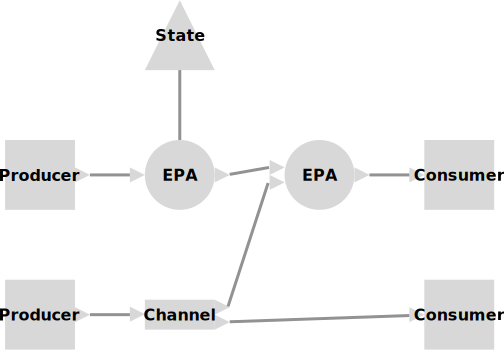
\includegraphics[scale=0.7]{images/epn.pdf}
\centering
\end{figure}

It is to be stressed that an EPN diagram is merely an abstraction, comprised of ``platform-independent definition elements''.
It does \emph{not} assume a distributed implementation.

After the introduction of the EPN concept, Etzion and Niblett \cite{Etzion:2010:EPA:1894960} lay out the ``[i]mplementation perspective'', in which the graph that the EPN is has to be materialized onto what are being called ``runtime artifacts''.
This results in a ``runtime system''.
Usually, there is no ``one-to-one correspondence'' between the processing elements of an EPN and the runtime artifacts of a respective implementation.
With regard to this, the authors describe two ``extremes'':

\begin{itemize}
\item
The entire EPN is be represented by one runtime artifact, resulting in one centralized runtime system.
\item
Each EPA is represented by one runtime artifact.
These distribute events between each other and ``can be placed on different server[s], allowing much of the [...] work to be performed in parallel.''
\end{itemize}

The second scenario can be considered a prime example for distributed EP, even though there are obviously many ways to map EPAs to runtime artifacts, several of which might also be considered distributed approaches.

In the chapter ``EPA assignment optimization'', which is concerned with mapping ``logical functions [i.e., EPAs] to physical runtime artifacts'', Etzion and Niblett \cite{Etzion:2010:EPA:1894960} mention parallel and distributed processing explicitly.
Parallel processing is considered ``[o]ne of the major ways to achieve [...] performance metrics''.
Then, three levels of parallelism are introduced, i.e., using multiple threads in one core, using multiple cores and using multiple machines.
However, finding out ``which activities should be run in parallel'' is considered a ``difficult'' challenge.
Regarding distributed processing, it is stated that ``moving the processing close to the producers and consumers'' constitutes an optimization method.
``Partitioning'', i.e., the practice of grouping EPAs that can ``execute together [i.e., in parallel]'', is introduced and considered ``key'' to both parallel and distributed execution.
``Stratification'', a partitioning approach in which EPAs are assigned to so-called ``strata'' is also described: ``If \lstinline{EPA1} produces events that are consumed by \lstinline{EPA2}, then \lstinline{EPA2} is placed in a higher stratum.''

Regarding the aforementioned challenge of parallel execution, noteworthy approaches (e.g., \cite{stratified, Farroukh:2009:PEP:1619258.1619269, Khandekar:2009:COS:1656980.1657002, Hirzel:2012:PCP:2335484.2335506}) have been proposed.
The previously mentioned optimization technique of ``moving the processing close to the producers and consumers'' poses yet another challenge, especially when it comes to mobile producers/consumers.
Interesting approaches to it (e.g., \cite{Pietzuch:2003:FEC:1515915.1515921, 1203579, Ottenwalder:2013:MOM:2488222.2488265}) have been presented.
Moreover, it appears that a good amount of the solutions to distributed EP proposed by academia are built upon loosely-coupled publish/subscribe systems (e.g., \cite{792159, Pietzuch:2003:FEC:1515915.1515921, 1203579, Farroukh:2009:PEP:1619258.1619269}), which constitute a related field of research.
Also, for the events of a stream to be put into time-based windows or for them to be temporally ordered, they need to be properly timestamped.
Timestamping is a well-studied challenge in distributed systems in general and constitutes yet another related field of research.
Many approaches have been proposed over time.
Liebig, Cilia and Buchmann \cite{792159} present an interesting solution that is specifically aimed at distributed EP, leveraging a combination of NTP-synchronized local clocks and heartbeat events.

\subsection{EP \& Quality of Service}
\label{sec:ep_qos}

Appel, Sachs and Buchmann \cite{quality} note that ``[f]uture software systems'' have to be ``responsive to events'' in order to ``adapt [...] software to enhance business processes''.
As an example, they mention software-controlled logistics processes that must be altered according to incoming updates on traffic.
It is stressed that in such a scenario, in which critical business processes are triggered by events, ``[t]he trust in such [...] systems depends to a large extent on the Quality of Service (QoS) provided by the underlying event system''.
The definition of QoS metrics as well as finding the means to monitor those is considered a ``major challenge''.

This section is structured as follows.
At first, QoS metrics that have been identified for publish/subscribe systems---which do mostly apply to EP, too---are described.
Afterwards, QoS metrics that are specific to SP or CEP are presented.

In their publication ``Quality of Service in Event-based Systems'', Appel, Sachs and Buchmann \cite{quality} point out that ``[f]or the [underlying] communication [...] the paradigm of choice is publish/subscribe'', i.e., many EP solutions are built upon publish/subscribe systems.
Thus, they refer to a paper by Behnel, Fiege and Mühl \cite{1648910}, in which QoS metrics for publish/subscribe-based systems are identified.
In this paper, publish/subscribe systems are defined as follows:

\emph{
``The system model of the publish-subscribe communication paradigm is surprisingly simple.
[... There are] three roles: publishers, subscribers and brokers.
Publishers [...] provide information, advertise it and publish notifications about it.
Subscribers [...] specify their interest and receive relevant information when it appears.
Brokers mediate between the two by selecting the right subscribers for each published notification. [...]
There can be a single centralized broker, a cluster of them or a distributed network of brokers.''}

It is to be noted, however, that Appel, Sachs and Buchmann \cite{quality} explicitly recommend to refrain from considering  generic QoS metrics.
They recommend to compile a list of specific, i.e, non-generic, QoS requirements for the EP solution in question ``rather than building a Swiss army knife EBS [i.e., event-based system] supporting all imaginable [...] QoS needs''.
Nevertheless, for the sake of completeness, the following paragraphs summarize some of the generic QoS metrics presented by Behnel, Fiege and Mühl \cite{1648910}. 

As said, even though the following QoS metrics were originally put together ``in the context of distributed and decentralized publish-subscribe systems'' \cite{1648910}, they do also apply to EP, since the underlying communication of many distributed EP solutions is based on the publish/subscribe paradigm.
In order to interpret these QoS metrics in the sense of EP, one can simply think of an EPN's event producers, event consumers and EPAs whenever publishers, subscribers and brokers of publish/subscribe systems are mentioned.
Furthermore, statements about publishers and subscribers do not only apply to event producers and event consumers, respectively, but also to EPAs, as these do also consume and produce event streams.
Notifications can be thought of as events.
For example, a statement such as, say, ``publishers annotate notifications they emit with priorities'' can be interpreted as ``event producers and EPAs annotate events they produce with priorities''. With no further ado, find below a summary of some of the QoS metrics proposed by Behnel, Fiege and Mühl \cite{1648910}.

\begin{description}
\item[Latency]
It is stated that ``[s]ubscribers request a publisher that is within a maximum latency bound''.
An ``end-to-end latency'' between a publisher and a subscriber ``depends on the number of [...] hops between them'' as well as on the time each broker takes to deal with a notification.
However, in a distributed setting, ``measured lower bounds'' may at best ``give hints'' about whether some latency requirement can be met---not ``absolute guarantees''.
Preallocating paths is mentioned as a way to deal with latency requirements.
\item[Bandwidth]
It is described that publishers announce upper/lower bounds regarding the stream they produce, whereas subscribers ``restrict the maximum stream of notifications they want to receive''.
It is recommended to consider bandwidth at the ``per-broker'' level.
Given that ``each broker knows the bandwidth it can make locally available to the infrastructure'', an upper-bound for an entire path can be estimated, allowing for routing ``based on the highest free bandwidth''.
\item[Message priorities]
It is proposed that publishers annotate the notations they produce with relative or absolute priorities, denoting their importance compared to other notifications produced either by themselves or elsewhere, respectively.
Subscribers, on the other hand, specify priorities regarding their subscriptions.
At the ``per-broker'' level, priorities ``can be used to control the local queues of each broker'', resulting in the ``end-to-end application'' of the priorities along the entire path.
This is, according to the authors, commonly implemented by letting notifications with higher priorities overtake those with lower priorities at each broker.
\item[Delivery guarantees]
While subscribers announce ``which notifications they must receive'', and where they are sensitive to duplicates, it is stated that publishers ``specify if subscribers must receive certain notifications''.
A simple approach that is mentioned is to simply let the system know which messages can be discarded.
More sophisticated approaches concern ``the completeness and duplication of delivery'', i.e., subscribers may receive notifications that are directed to them ``at least once'', ``at most once'' or ``exactly once''.
While meshing is listed as a way to achieve ``at least once'', it comes at the price of ``increasing the message overhead''.
Disconnected subscribers are yet ``[a]nother problem'', as they might stay disconnected, in which case ``at least once'' cannot be guaranteed, no matter how long the notifications are buffered.
\item[Notification order]
It is explained that ``[t]he order in which notifications arrive'' is of significance in some cases while it is not in other cases.
With centralized ordering, ``ordering is [considered] easy to achieve''.
However, ``distributed ordering of events coming from different sources'' is described as problematic.
Deploying a ``central broker to enforce a global ordering'' is mentioned as a ``generic approach'' to tackle this challenge, imposing a ``limit'' on the ``scalability of the overall infrastructure'', though.
\item[Validity interval]
The importance of the infrastructure to know ``how long a notification stays valid'' is stressed.
It is explained that this is specified either ``in terms of time'' or ``by the arrival of later messages''.
Using a specification based on ``follow-up messages'' to express that ``only the most recent event is of interest'' is mentioned as an example of the latter.
This is called an ``efficient approach'', as it allows for the infrastructure to ``shorten its queues in high traffic situations''.
\end{description}

When interpreting the above list of QoS metrics in terms of EP, it becomes evident that these metrics can be applied to both SP as well as CEP.
(As said, brokers are to be thought of as EPAs, and it has not been specfied whether these EPAs perform SP or CEP operations.)
However, there are QoS metrics that specifically apply to either SP or CEP.
Some of them have been identified in the paper ``From Calls to Events: Architecting Future BPM Systems'' \cite{Buchmann:2012:CEA:2413516.2413519} by Buchmann et al., several of which are summarized below.

SP-specific QoS metrics listed in section ``QoS of Stream Processing'' \cite{Buchmann:2012:CEA:2413516.2413519} include:

\begin{description}
\item[Timeliness]
One the one hand, it is stated that applications relying on SP ``typically have timing constraints to meet'', thus, the timeliness of the ``continuous processing of incoming events'' is considered ``one of the most relevant QoS requirements''.
On the other hand, many of these applications are said to ``tolerate approximate results''.
According to the authors, these circumstances suggest a ``common'' ``trade-off'', i.e., ``accuracy for timeliness''.
To the best of my understanding, an example of this trade-off would be favoring some less precise filter that therefore executes quickly over some more precise and more time-consuming filter.
\item[Throughput]
With regards to timeliness, ``achievable throughput'' is considered a ``closely related QoS metric''.
SP solutions are said to ``attempt to optimize'' their ``continuous query execution'' in order to achieve maximum throughput.
As load shedding is considered to ``often'' be the ``only practical approach'', the result is, again, the ``trade-off of accuracy for timeliness''.
\item[Order]
Whether events may be processed out of order is listed as an ``application dependent'' ``issue''.
\end{description}

CEP-specific QoS metrics listed in section ``QoS of Event Composition'' \cite{Buchmann:2012:CEA:2413516.2413519} include:

\begin{description}
\item[Order]
Establishing an ``ordering between events'' can be considered the most important QoS metric, as ``achievable QoS [...] depends largely on the possibility'' to be able to do so.
As an example of an operator that requires events to be ordered, the \lstinline{sequence} operator, ``which is part of most [CEP] event algebras'', is mentioned.
Furthermore, it is stated that the ``natural ordering'' is time-based, which, according to the authors, is no problem if ``there is only one central clock'' as well as only one event occurring per clock tick.
If, however, there may be ``multiple events'' occurring at the same point in time, being ``time-stamped by different clocks'', establishing a total order is said to be impossible.
Lastly, it is explained that the granularity of timestamps plays a major role:
Events that might have been distinguishable with fine-grained timestamps might no be distinguishable when being timestamped more coarsely.
\item[Delay/loss of messages]
The delay or loss of messages is described as a ``source of ambiguity''.
As an example, it is explained that it is impossible to determine that an event ``did not occur in a given interval'' unless it can be asserted that the event in question is neither delayed nor lost.
With regard to bounded networks, the authors refer to the 2g-precedence model as a possibility to tackle this challenge.
With regard to unbounded networks, ``such as the internet'', they refer to a paper called ``Event composition in time-dependent distributed systems'' \cite{792159}. (This paper also contains an explanation of the 2g-precendce model.)
\end{description}

\newpage

\section{EventScala}
\label{sec:eventscala}


\subsection{Case Class Representation}
\label{sec:case_class_rep}

At the heart of the EventScala framework is the case class representation of queries.
Thanks to it, EventScala's DSL and EventScala's execution engine can be thought of as separate modules that do not depend on each other in any way.
On the one hand, using the DSL to express a query results in the case class representation of that query.
On the other hand, running a query using the execution engine requires a case class representation of said query.
However, a case class representation of a query does neither have to be obtained using the DSL nor it have to be executed using the execution engine.
One could, for example, use EventScala's DSL to obtain the case class representation of a query and then generate a SQL-like string from it to execute it using, say, Esper.
Likewise, one could develop a different DSL or even type out the case class representation of a query by hand and then pass it to EventScala's execution engine to be run.
Essentially, EventScala's case class representation is a type-safe and platform-independent way to encode queries for EP systems in Scala.

In this section, EventScala's case class representation is presented in great detail.
To this end, the hierarchy and structure of the traits and case classes that make up the case class representation of queries is explained.

At the top of the hierarchy is the \lstinline{Query} trait, which only specifies that extending classes have to have a field called \lstinline{requirements}, representing a set of QoS requirements that were specified for the respective query.
(Refer to the end of this section as well as to section \ref{sec:qos} for more information on QoS requirements in EventScala.)

As described in section \ref{sec:event_processing}, events are commonly represented by tuples of values, i.e., an event consisting of n values would be represented by a n-tuple.
In EventScala, an event consists of at least one element and at most six elements.
Analogously, the \lstinline{Query} trait is extended by the traits \lstinline{Query1}, \lstinline{Query2}, ..., \lstinline{Query6}, each representing a query that results in a stream of events consisting of 1, 2, ..., 6 elements, respectively.
The traits \lstinline{Query1}, \lstinline{Query2}, ..., \lstinline{Query6} do not specify any additional fields.
They do, however, take 1, 2, ..., 6 type parameters, respectively, specifying the types of the elements of the events of the respective streams they represent.
\lstinline{Query2[String, Int]} is, for example, the type of a query that results in a stream of events which consist of two elements: a \lstinline{String} and an \lstinline{Int}.

A query usually consists of nested applications of operators over primitives.
For example, one might subscribe to a stream of events consisting of a single \lstinline{Int}, resulting in a \lstinline{Query1[Int]}, as well as to a stream of events consisting of two \lstinline{String}s, resulting in a \lstinline{Query2[String, String]}.
One might then apply the \lstinline{join} operator to these two stream subscriptions, resulting in a \lstinline{Query3[Int, String, String]}.
Afterwards, one could decide to drop the second \lstinline{String} using the \lstinline{dropElem3} operator, resulting in a \lstinline{Query2[Int, String]}.
When picturing this query as a graph (as illustrated in figure \ref{fig:query}), the \lstinline{dropElem3} operator would be the root node, having one child node, i.e., the \lstinline{join} operator, which, in turn, would have two child nodes, i.e., the two stream subscriptions, which would be represented by the leaves of the graph.
(In fact, this graph precisely resembles the graph of concurrently executing nodes that would be created if the query were run by EventScala's execution engine.)

Analogously, the application of the \lstinline{dropElem3} operator can be thought of as a unary query---unary in the sense that it has one subquery.
Furthermore, the application of the \lstinline{join} operator can be thought of as a binary query---binary in the sense that it has two subqueries.
Lastly, the subscription to a stream can be thought of as a leaf query---leaf in the sense that it has no child queries.
As a matter of fact, in EventScala, every query can be classified into being either a leaf, a unary or a binary query.
Therefore, there exist three traits \lstinline{LeafQuery}, \lstinline{UnaryQuery} (specifying one field,  \lstinline{sq} (\lstinline{s}ub\lstinline{q}uery), of type \lstinline{Query}) and \lstinline{BinaryQuery} (specifying two fields, \lstinline{sq1} and \lstinline{sq2}, both of type \lstinline{Query}).
All three traits extend the trait \lstinline{Query}.

\begin{figure}
\caption{A conceptual depiction of a \lstinline{Query}}
\label{fig:query}
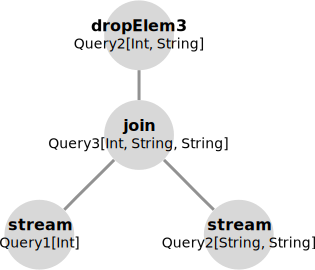
\includegraphics[scale=0.7]{images/query.pdf}
\centering
\end{figure}

In the previous paragraph, it has been hinted that in EventScala, one might subscribe to streams or make use of the operators \lstinline{join} or \lstinline{dropElem3}.
For the sake of completeness, find below the list of all primitives (i.e., leaf queries) and operators (i.e., unary and binary queries) available.

Leaf queries, i.e., traits extending the \lstinline{LeafQuery} trait:

\begin{description}
\item[StreamQuery]
A \lstinline{StreamQuery} expresses a subscription to a stream.
The trait \lstinline{StreamQuery} specifies one field of type \lstinline{String}, \lstinline{publisherName}, for the name of the publisher that is the source of the stream.
\item[SequenceQuery]
A \lstinline{SequenceQuery} expresses a subscription to two streams with the CEP operator \lstinline{sequence} being applied to them.
The trait \lstinline{SequenceQuery} specifies two fields of type \lstinline{NStream}, \lstinline{s1} and \lstinline{s2}.
A \lstinline{NStream} is essentially a \lstinline{Stream}, however, it is ``\lstinline{N}ot a query'', i.e., not extending the trait \lstinline{Query}.
If \lstinline{NStream} would be a query, then \lstinline{s1} and \lstinline{s2} would represent the subqueries of a \lstinline{SequenceQuery}, which would make it a binary query rather than a leaf query.
\end{description}

Unary queries, i.e., traits extending the \lstinline{UnaryQuery} trait:

\begin{description}
\item[FilterQuery]
A \lstinline{FilterQuery} expresses the application of the SP operator \lstinline{where}.
The \lstinline{FilterQuery} trait specifies one field of type \lstinline{Event => Boolean}, \lstinline{cond}, for the filter predicate.
The field for the subquery representing the operator's input stream is specified by the extending classes.
\item[DropElemQuery]
A \lstinline{DropElemQuery} expresses the application of the operator that EventScala offers instead of the EP operator \lstinline{select}.
While \lstinline{select} lets one select which elements of the events of the operator's input stream to keep, the \lstinline{dropElem} operator lets one specify which element to drop.
The \lstinline{DropElemQuery} trait specifies no fields.
Which element of the events of the operator's input stream is to be dropped is specified through the extending classes' names, e.g., \lstinline{DropElem1Of2}.
\item[SelfJoinQuery]
A \lstinline{SelfJoinQuery} expresses the application of the SP operator \lstinline{join} but with one stream representing both of the operator's input streams.
The \lstinline{SelfJoinQuery} trait specifies two fields of type \lstinline{Window}, \lstinline{w1} and \lstinline{w2}, for the windows that are applied to the operator's input streams.
The field for the subquery representing both of the operator's input streams is specified by the extending classes.
\end{description}

Binary queries, i.e., traits extending the \lstinline{BinaryQuery} trait:

\begin{description}
\item[JoinQuery]
A \lstinline{JoinQuery} expresses the application of the SP operator \lstinline{join}.
The \lstinline{JoinQuery} trait specifies two fields of type \lstinline{Window}, \lstinline{w1} and \lstinline{w2}, for the windows that are applied to the operator's input streams.
The fields for the two subqueries representing the operator's input streams are specified by the extending classes.
\item[ConjunctionQuery]
A \lstinline{ConjunctionQuery} expresses the application of the CEP operator \lstinline{and}.
The \lstinline{ConjunctionQuery} trait specifies no fields.
The fields for the two subqueries representing the operator's input streams are specified by the extending classes.
\item[DinjunctionQuery]
A \lstinline{DisjunctionQuery} expresses the application of the CEP operator \lstinline{or}.
The \lstinline{DisjunctionQuery} trait specifies no fields.
The fields for the two subqueries representing the operator's input streams are specified by the extending classes.
\end{description}

Up to this point, a hierarchy of traits but not one case class has been presented.
The case class representation of a query is, however, made up of (possibly nested) case class instances.
These case classes have the following in common:

\begin{itemize}
\item
They extend exactly one of the traits \lstinline{Query1}, \lstinline{Query2}, ..., \lstinline{Query6}, indicating the number and types of the elements of the events of the stream they represent.
\item
They extend exactly one of the traits \lstinline{StreamQuery}, \lstinline{SequenceQuery}, \lstinline{FilterQuery}, \lstinline{DropElemQuery}, \lstinline{SelfJoinQuery}, \lstinline{JoinQuery}, \lstinline{ConjunctionQuery} or \lstinline{DisjunctionQuery}, indicating what kind of primitive or operator application they represent.
\end{itemize}

For example, the case class \lstinline{Stream1[A]} extends the trait \lstinline{Query1[A]}, indicating that it represents a stream of events consisting of \lstinline{1} element of the generic type \lstinline{A}, as well as the trait \lstinline{StreamQuery}, indicating that it represents a subscription to a stream, i.e., a primitive.
It has a field \lstinline{publisherName} as specified by the trait \lstinline{StreamQuery} as well as a field \lstinline{requirements} as specified by the trait \lstinline{Query}.
\lstinline{Conjunction12[A, B, C]}, to provide another example, extends the trait \lstinline{Query3[A, B, C]}, indicating that it represents a stream of events consisting of 3 elements of the generic types \lstinline{A}, \lstinline{B} and \lstinline{C}, respectively, as well as the trait \lstinline{ConjunctionQuery}, indicating that it represents an application of the \lstinline{and} operator.
Obviously, it also has the field \lstinline{requirements}.

More interestingly, though, the case class \lstinline{Conjunction12[A, B, C]} also has two fields (\lstinline{sq1} of type \lstinline{Query1[A]} and \lstinline{sq2} of type \lstinline{Query2[B, C]}) for the subqueries representing the \lstinline{and} operator's two input streams, which---against one's intuition---are not specified in the \lstinline{ConjunctionQuery} trait.
The reason for this is that while every case class extending \lstinline{ConjunctionQuery} does have two fields named \lstinline{sq1} and \lstinline{sq2}, the two fields' types are always different.
For the case class \lstinline{Conjunction11[A, B]}, their types are \lstinline{Query1[A]} and \lstinline{Query1[B]}, respectively, and for \lstinline{Conjunction21[A, B, C]}, to provide another example, they are \lstinline{Query2[A, B]} and \lstinline{Query1[C]}, respectively.
This hints at the biggest shortcoming of EventScala:
As it is not possible to abstract over the length of type parameter lists in Scala, one cannot define one trait (like \lstinline{trait Query[A, B, ...]}) for queries in general, but has to define one separate trait (e.g., \lstinline{Query1[A]}, \lstinline{Query2[A, B]}, and so forth) for queries representing streams of events consisting of one element, two elements, and so forth.
(Tuples actually suffer from the same shortcoming: \lstinline{Tuple1[+T1]}, \lstinline{Tuple2[+T1, +T2]}, and so forth, are all defined separately in the Scala standard library.)
To avoid a ridiculous amount of code repetition, in EventScala, events can consist of at most six elements.
Still, this seemingly small number does not only call for the six separate traits \lstinline{Query1[A]} to \lstinline{Query6[A, B, C, D, E, F]}, but also for 15 separate case classes extending the \lstinline{SequenceQuery} trait as well as, to provide the most extreme example, for 36 case classes extending the \lstinline{DisjunctionQuery} trait.
Any future work on this project should aim to solve this issue, maybe by representing events and queries with \lstinline{HList}s, which encode the types of their members (which can be \lstinline{H}eterogenuous, i.e., of different types) in their type. They are provided by the popular Scala library Shapeless \cite{shapeless}, a ``type class and dependent type based generic programming library for Scala''.

At this point, EventScala's case class representation has been explained to an extent that an example query in case class representation (listing \ref{lst:query}) can be presented.

\begin{lstlisting}[
caption={Case class representation of the query depicted in figure \ref{fig:query}},
label={lst:query}]
val sampleQuery1: Query2[Int, String] =
  DropElem3Of3[Int, String, String](
    Join12[Int, String, String](
      Stream1[Int]("X", Set.empty),
      Stream2[String, String]("Y", Set.empty),
      SlidingTime(42),       // Sliding window of 42 seconds
      TumblingInstances(21), // Tumbling window of 21 events
      Set.empty),
    Set.empty)
\end{lstlisting}

The avid reader has certainly noticed that this is the case class representation of the query that has been informally described and illustrated as a graph (figure \ref{fig:query}) previously in this section.
It is to be stressed that this is a type-safe representation of said query.
(This point will be discussed in detail in section \ref{sec:dsl}.)
Also, it is to be mentioned that it is also a platform-independent representation, i.e., it neither encodes data specific to the DSL that generated it nor does it encode data that is specific to the EP solution that will execute it.

Lastly, as the title of this thesis suggests, EventScala is a quality-of-service-oriented approach to EP.
As such, it allows for QoS requirements, i.e., run-time requirements, to be expressed with each query.
One might have noticed that \lstinline{sampleQuery1} (listing \ref{lst:query}) contains the expression \lstinline{Set.empty} four times.
At these four points, it would have been possible to define a set of requirements (of type \lstinline{Set[Requirement]}).
When picturing the query as a graph once again, it becomes clear that requirements can be defined over every node of the graph.
EventScala features two kinds of requirements, \lstinline{FrequencyRequirement}s and \lstinline{LatencyRequirement}s.
(These will be discussed in greater detail in section \ref{sec:qos}.)
It is to be noted, however, that the case classes representing these requirements are not platform-independent.
This is due to the fact that they do not just contain the specification of the respective requirement.
They also embody a callback closure that defines what to do whenever the respective requirement is not met during the execution of the query.
The fact that this callback closure is being passed data about the processing node that is responsible for executing the respective (sub)query is what breaks platform independence.
Therefore, queries containing QoS requirements are bound to be run by EventScala's execution engine.
As there are---to the best of my knowledge---no other EP solutions that allow for the definition or execution of per-query QoS requirements, this does not constitute a real limitation.
Listing \ref{lst:query2} shows another example query, representing a stream subscription that is being applied to a filter, with the stream being required to emit at least 2 events per 5 seconds.

\begin{lstlisting}[
caption={Case class representation of a query that specifies a QoS requirement},
label={lst:query2}]
val sampleQuery2: Query2[Int, Boolean] =
  Filter2[Int, Boolean](
    Stream2[Int, Boolean](
      "Z",
      // If not at least 2 events are emitted every 5 seconds,
      // "Problem!" will be printed to the console.
      Set(FrequencyRequirement(GreaterEqual, 2, 5, _ => println("Problem!")))),
    // This filter predicate does not filter out any event. :)
    _ => true,
    // No QoS requirements are defined over the filter.
    Set.empty)
\end{lstlisting}

\subsection{Domain-Specific Language}
\label{sec:dsl}

EventScala's DSL for expressing queries for EP systems sets out to achieve in the domain of EP what ScalaQL \cite{Spiewak:2009:SLD:2127907.2127923} and other DSLs achieved for relational databases, i.e., ``statically eliminating [...] runtime issues'' \cite{Spiewak:2009:SLD:2127907.2127923} caused by ``syntactically incorrect or ill-typed queries'' \cite{Leijen:1999:DSE:331960.331977}.
EventScala's DSL can be classified as an internal DSL.
With EventScala being a Scala framework, its host language is obviously Scala.

This section is structured as followed. 
At first, the DSL is presented from a user's perspective, i.e., an overview of its features is given and advantages are pointed out.
Then, notable parts of its implementation are discussed, e.g., the use of Scala features such as implicit conversion \cite{pimp}.

In the previous section, it has already been revealed which primitives and operators are supported by EventScala.
In the listings \ref{lst:dsl_leaf}, \ref{lst:dsl_unary}, \ref{lst:dsl_binary} and \ref{lst:dsl_nested}, it will be shown how the DSL can be used to express queries made up of these primitives and operators, i.e., how the DSL can be used to express leaf, unary and binary queries.

\begin{lstlisting}[
caption={Primitives, i.e., leaf queries},
label={lst:dsl_leaf}]
// Subscription to a stream
// of events of type `Int` from A
val stream1: Query1[Int] =
  // Here, the type has to be explicitly annotated:
  stream[Int]("A")

// Subscription to a stream
// of events of type `String, String` from B
val stream2: Query2[String, String] =
  stream[String, String]("B")

// Subscription to two streams
// of events of type `Int` and `Boolean`, respectively,
// with the CEP operator `sequence` applied to them
val sequence1: Query2[Int, Boolean] =
  // Here, the types have to be explicitly annotated:
  sequence(
    nStream[Int]("C") ->
    nStream[Boolean]("D"))

// Subscription to two streams
// of events of type `Int, Int` and `Int`, respectively,
// with the CEP operator `sequence` applied to them
val sequence2: Query3[Int, Int, Int] =
  sequence(
    nStream[Int, Int]("E") ->
    nStream[Int]("F"))
\end{lstlisting}

\begin{lstlisting}[
caption={Application of unary operators, i.e., unary queries},
label={lst:dsl_unary}]
// Application of the SP operator `where`
// to `stream1` (`Query1[Int]`)
val filter1: Query1[Int] =
  stream1.where(_ % 2 == 0)
  // Alternatively: `stream1 where (_ % 2 == 0)`

// Application of the SP operator `where`
// to `sequence2` (`Query3[Int, Int, Int]`)
val filter2: Query3[Int, Int, Int] =
  sequence2.where((e1, _, e3) => e1 < e3)

// Application of the SP operator `dropElem2`
// to `stream2` (`Query2[String, String]`)
val dropElem1: Query1[String] =
  stream2.dropElem2()
  // Alternatively: stream2 dropElem2()

// Application of the SP operator `dropElem1`
// to `sequence1` (`Query2[Int, Boolean]`)
val dropElem2: Query1[Boolean] =
  sequence1.dropElem1()

// Application of the SP operator `selfJoin`
// to `stream2` (`Query2[String, String]`)
val selfJoin1: Query4[String, String, String, String] =
  stream2.selfJoin(
    slidingWindow(42.instances), // Alternatively: `42 instances`
    tumblingWindow(42.seconds))  // Alternatively: `42 seconds`

// Application of the SP operator `selfJoin`
// to `sequence1` (`Query2[Int, Boolean]`)
val selfJoin2: Query4[Int, Boolean, Int, Boolean] =
  sequence1.selfJoin(
    tumblingWindow(42.instances),
    slidingWindow(42.seconds))
\end{lstlisting}

\begin{lstlisting}[
caption={Application of binary operators, i.e., binary queries},
label={lst:dsl_binary}]
// Application of the SP operator `join`
// to `stream1` (`Query1[Int]`)
// and `stream2` (`Query2[String, String]`)
val join1: Query3[Int, String, String] =
  stream1.join(
    stream2,
    slidingWindow(42.instances),
    tumblingWindow(42.seconds))

// Application of the SP operator `join`
// to `sequence1` (`Query2[Int, Boolean]`)
// and `sequence2` (`Query3[Int, Int, Int]`)
val join2: Query5[Int, Boolean, Int, Int, Int] =
  sequence1.join(
    sequence2,
    slidingWindow(42.instances),
    tumblingWindow(42.seconds))

// Application of the CEP operator `and`
// to `stream2` (`Query2[String, String]`)
// and `stream1` (`Query1[Int]`)
val conjunction1: Query3[String, String, Int] =
  stream2.and(stream1)
  // Alternatively: `stream2 and stream1`

// Application of the CEP operator `and`
// to `sequence1` (`Query2[Int, Boolean]`)
// and `sequence2` (`Query3[Int, Int, Int]`)
val conjunction2: Query5[Int, Boolean, Int, Int, Int] =
  sequence1.and(sequence2)
  // Alternatively: `sequence1 and sequence2`

// Application of the CEP operator `or`
// to `stream1` (`Query1[Int]`)
// and `stream2` (`Query2[String, String]`)
val disjunction1: Query2[Either[Int, String], Either[X, String]] =
  stream1.or(stream2)
  // Alternatively: `stream1 or stream2`

// Application of the CEP operator `or`
// to `sequence2` (`Query3[Int, Int, Int]`)
// and `sequence1` (`Query2[Int, Boolean]`)
val disjunction2: Query3[Either[Int, Int], Either[Int, Boolean], Either[Int, X]] =
  sequence2.or(sequence1)
  // Alternatively: `sequence1 or sequence2`
\end{lstlisting}

\begin{lstlisting}[
caption={Nested queries},
label={lst:dsl_nested}]
// Nested application
// of 3 unary and 3 binary operators
// to 4 primitives
val nested1: Query3[Either[Int, String], Either[Int, X], Either[Float, X]] =
  stream[Int]("A")
    .join(
      stream[Int]("B"),
      slidingWindow(2.seconds),
      slidingWindow(2.seconds))
    .where(_ < _)
    .dropElem1()
    .selfJoin(
      tumblingWindow(1.instances),
      tumblingWindow(1.instances))
    .and(stream[Float]("C"))
    .or(stream[String]("D"))

// Nested application
// of 2 binary operators
// to 3 (!) primitives
val nested2: Query4[Int, Int, Float, String] =
  stream[Int]("A")
    .and(stream[Int]("B"))
    .join(
      sequence(
        nStream[Float]("C") ->
        nStream[String]("D")),
      slidingWindow(3.seconds),
      slidingWindow(3.seconds))
\end{lstlisting}

Furthermore, the section presenting the case class representation of queries also revealed that EventScala supports queries to be annotated with QoS requirements, i.e., \lstinline{FrequencyRequirement}s and  \lstinline{LatencyRequirement}s.
As already mentioned, every query, including arbitrarily deeply nested subqueries, can be annotated with an arbitrary amount of QoS requirements.
In listing \ref{lst:dsl_qos}, it is demonstrated how requirements are expressed using the DSL.
It is shown how two of the subqueries of the query \lstinline{nested1} from listing \ref{lst:dsl_nested} are annotated with requirements.

\begin{lstlisting}[
caption={Nested queries that specify QoS requirements},
label={lst:dsl_qos}]
val nested1WithQos: Query3[Either[Int, String], Either[Int, X], Either[Float, X]] =
  stream[Int]("A")
  .join(
    stream[Int]("B"),
    slidingWindow(2.seconds),
    slidingWindow(2.seconds))
  .where(_ < _)
  .dropElem1(
    // `LatencyRequirement`
    latency < timespan(1.milliseconds) otherwise { (nodeData) =>
      println(s"Events reach node `${nodeData.name}` too slowly!") })
  .selfJoin(
    tumblingWindow(1.instances),
    tumblingWindow(1.instances),
    // `FrequencyRequirement`s
    frequency > ratio( 3.instances,  5.seconds) otherwise { (nodeData) =>
      println(s"Node `${nodeData.name}` emits too few events!") },
    frequency < ratio(12.instances, 15.seconds) otherwise { (nodeData) =>
      println(s"Node `${nodeData.name}` emits too many events!") })
  .and(stream[Float]("C"))
  .or(stream[String]("D"))
\end{lstlisting}

At this point it becomes apparent why the definition of QoS requirements in EventScala's DSL (and, by extension, EventScala's case class representation) is platform-specific:
A QoS requirement always defines a callback closure that expects to be invoked with data, i.e., \lstinline{nodeData}, that is specific to EventScala's execution engine.
The \lstinline{nodeData} parameter can be explained as follows.
Each of a query's subqueries (and, in turn, each of its subqueries) is mapped to one processing node when run by the execution engine.
Whenever one of the requirements of such a query cannot be met during run-time, the callback closure of the respective requirement is called.
This closure is invoked with run-time data about the processing node that executes the respective query.
This run-time data is represented by an instance of the case class \lstinline{NodeData}.

Expressing EP queries using EventScala's DSL has many advantages over expressing them in the form of unstructured strings, including the ones listed below:

\begin{description}
\item[Syntax]
Obvious but nevertheless very important is the fact that syntactically incorrect queries would fail to compile instead of causing run-time errors.
For example, forgetting the dot before adding another method call to the chain or misspelling a method's name would cause a compile-time error.
\item[Type-safety]
The type of a query encodes the number and types of the elements of the events of the stream represented by it, e.g., a query of type \lstinline{Query2[Int, String]} represents a stream of events with two elements of type \lstinline{Int} and \lstinline{String}, respectively.
This information is used to provide static safeguards against a variety of malformed queries, for example:
\begin{itemize}
\item
Type-safety of the \lstinline{filter} operator:
The \lstinline{where} method takes a Scala closure that represents the filter predicate.
The number and types of the parameters of that closure match the number and types of the elements of the events of the stream that is represented by the respective query.
For example, given a query of type \lstinline{Query2[Int, String]}, the programmer has to supply a closure with exactly two parameters of type \lstinline{Int} and \lstinline{String}, respectively.
By extension, it is guaranteed that within the closure's body, these parameters are treated as an \lstinline{Int} and a \lstinline{String}, respectively, e.g., calling the \lstinline{String} method \lstinline{capitalize} on the first parameter would cause a compile-time error.
\item
Type-safety of the \lstinline{dropElem} operator:
Which ones of the \lstinline{dropElem} methods are available depends on the number of elements of the events of the stream represented by the query in question.
For example, on a \lstinline{Query1}, not one \lstinline{dropElem} method can be invoked.
Given a \lstinline{Query2}, to provide another example, \lstinline{dropElem1} and \lstinline{dropElem2} can be called.
Calling \lstinline{dropElem3} on a \lstinline{Query2}, however, results in a compile-time error.
\item
Type-safety of the operators \lstinline{selfJoin}, \lstinline{join} and \lstinline{and}:
EventScala supports up to six elements per event.
Therefore, the application of the operators \lstinline{selfJoin}, \lstinline{join} and \lstinline{and} is only possible if the resulting query represents a stream of events with at most six elements.
For example, when calling the \lstinline{join} method on a \lstinline{Query4}, only a \lstinline{Query1} or a \lstinline{Query2} can be passed to it as the second operand of the \lstinline{join} operator.
\end{itemize}
\item[Tooling]
As the DSL is an internal DSL that is embedded into Scala, every query expressed in it is a Scala expression.
As a consequence, IDEs and other tools from the Scala ecosystem can be leveraged when expressing queries using the DSL.
For example, one could benefit from the static safeguards listed above without ever manually hitting the compile button, as IDEs such as JetBrains IntelliJ IDEA \cite{idea} continuously perform static analysis while typing.
\end{description}

Obviously, this list of advantages could have been presented earlier, i.e., as part of the section on EventScala's case class representation of queries.
All of the listed benefits also apply to the case class representation, since the DSL can be viewed as syntactic sugar for it.

Finally, as the DSL's usage has been demonstrated and its advantages have been pointed out, the remainder of this section discusses how it is implemented, i.e., some of the leveraged patterns and Scala features are described.

In EventScala's DSL, operators are represented by methods.
It might look as if these methods were defined on the traits \lstinline{Query1}, \lstinline{Query2}, ..., \lstinline{Query6}.
Assuming a value \lstinline{q} of type \lstinline{Query2}, one can, for example, write \lstinline{q.dropElem1()}, which suggests that \lstinline{dropElem1} is a method of \lstinline{Query2}.
This would, however, violate the separation of data and logic.
Therefore, it is to be stressed that \lstinline{Query2}---along with every trait or case class that is part of EventScala's case class representation---does not come with any logic whatsoever, i.e., no methods are defined or implemented.

In order to make method calls such as \lstinline{q.dropElem1()} possible, the DSL heavily relies on one of Scala's advanced language features, implicit conversion.
In a blog post called ``Pimp my Library'' \cite{pimp}, Martin Odersky, the original designer of the Scala programming language, explains this feature.
In the context of this thesis, it is sufficient to understand the following use case: Whenever a value of type \lstinline{X} is required but instead a value of type \lstinline{Y} is being supplied, the compiler tries to find a function that is capable of converting the \lstinline{Y} value to a \lstinline{X} value.
For this to work, the function has to be in scope, it has to be marked with the \lstinline{implicit} keyword and its signature has to be \lstinline{Y => X}.
As an example, Odersky introduces \lstinline{x} of type \lstinline{Array[Int]} and assigns \lstinline{x} to \lstinline{v}, a variable of type \lstinline{String}.
Obviously, this would normally result in a compile-time error.
However, it does not, since the function depicted in listing \ref{lst:implicit} is in scope.

\begin{lstlisting}[
caption={Implicit conversion function \cite{pimp}},
label={lst:implicit}]
implicit def array2string[T](x: Array[T]) = x.toString
\end{lstlisting}

At this point it becomes apparent why method calls such as \lstinline{q.dropElem1()} do not result in a compile-time error:
\lstinline{q} is of type \lstinline{Query2}, which neither defines nor implements the method \lstinline{dropElem1}.
However, there is a case class \lstinline{Query2Helper} which does have this method.
There also is an implicit conversion function that takes a \lstinline{Query2} and returns a \lstinline{Query2Helper}.
Needless to say, for each trait \lstinline{Query1}, \lstinline{Query2}, ..., \lstinline{Query6}, there is a case class \lstinline{Query1Helper}, \lstinline{Query2Helper}, ..., \lstinline{Query6Helper}, respectively, as well as a respective implicit conversion function in place.

This is basically a simplification of an approach proposed by Debasish Ghosh in his book ``DSLs in Action'' \cite{Ghosh:2010:DA:1965333}.
In chapter 6.4 ``Building a DSL that creates trades'', he uses a ``[s]equence of implicit conversions'' and the ``subsequent creation of helper objects'' to construct a tuple that represents something called a fixed income trade.
This pattern can be described as follows:
The DSL is used to construct a tuple.
The tuple's first element should be of type \lstinline{A}, the second one of type \lstinline{B}, the third one of type \lstinline{C}, etc.
Helper classes \lstinline{AHelper}, \lstinline{ABHelper}, \lstinline{ABCHelper}, etc. as well as the respective implicit conversion functions with the signatures \lstinline{A => AHelper}, \lstinline{(A, B) => ABHelper}, \lstinline{(A, B, C) => ABCHelper}, etc. are defined.
\lstinline{AHelper} has a \lstinline{method1} that takes a \lstinline{B} and returns an \lstinline{(A, B)}, \lstinline{ABHelper} has a \lstinline{method2} that takes a \lstinline{C} and returns an \lstinline{(A, B, C)}, and so forth.
This pattern allows for expressions such as \lstinline{a method1 b method2 c /* ... */} (with \lstinline{a} being an \lstinline{A}, \lstinline{b} being a \lstinline{B}, and so forth).
As said, Ghosh \cite{Ghosh:2010:DA:1965333} presents this pattern along with an example DSL is based upon it.
He demonstrates how the expression \lstinline{200 discount_bonds IBM for_client NOMURA on NYSE at 72.ccy(USD)} can be used to obtain a tuple that represents a fixed income trade, i.e., \lstinline{((72, USD), NYSE, NOMURA, 200, IBM)}.

Another Scala feature that the DSL heavily relies upon is operator overloading.
Technically, however, Scala does not support operator overloading, as it does not even have operators.
Instead, what seem to be operators are actually methods.
The arithmetic operator \lstinline{+} that is defined over two \lstinline{Int}s, for instance, is really just the method \lstinline{abstract def +(x: Int): Int} of the abstract class \lstinline{Int}.
As such, the two expressions \lstinline{40 + 2} and \lstinline{40.+(2)} are actually equivalent.
With many characters being legal identifiers that can be used as method names, e.g., \lstinline{+}, \lstinline{>}, \lstinline{<}, \lstinline{|}, overloading an operator in Scala is nothing more than defining a method.
This feature is used throughout the DSL.
For example, in order to construct a \lstinline{FrequencyRequirement}, one might write \lstinline{frequency > ratio(/* ... */) /* ... */}.
Calling the function \lstinline{frequency} returns a case object called \lstinline{FrequencyHelper}, which defines a bunch of methods, including \lstinline{>}, \lstinline{>=}, \lstinline{<}, \lstinline{<=}, etc., all of which take one argument of type \lstinline{Ratio}.

Lastly, variable-length argument lists (also known as varargs) constitute yet another Scala feature that is used throughout the DSL.
Varargs are, for instance, used to syntactically reflect the fact that queries in EventScala can be annotated with zero or more QoS requirements.
Therefore, \lstinline{Requirement*} is the type of the last parameter of every method of the DSL that returns a query.
The \lstinline{stream[A]} method, for example, specifies two parameters, i.e., \lstinline{publisherName} of type \lstinline{String} and \lstinline{requirements} of type \lstinline{Requirement*}.
As a consequence, this method might be supplied with no requirement, e.g., \lstinline{stream[Int]("X")}, with one requirement, e.g., \lstinline{stream[Int]("X", r1)}, with two requirements, e.g., \lstinline{stream[Int]("X", r1, r2)}, etc. (with \lstinline{r1}, \lstinline{r2}, etc. being of type \lstinline{Requirement}).
If the DSL would not rely on varargs but simply use \lstinline{Set[Requirement]} as the type of the \lstinline{requirements} parameter---as it is the case in the case class representation---these method calls would look much more verbose:
\lstinline{stream[Int]("X", Set.empty)}, \lstinline{stream[Int]("X", Set(r1))}, \lstinline{stream[Int]("X", Set(r1, r2))}, etc.

\subsection{Execution Engine}
\label{sec:execution_engine}

EventScala does not only offer a type-safe case class representation of EP queries and a DSL to generate the former, it also offers a way to execute such queries. As the title of this thesis suggests, EventScala's execution engine allows for running queries in a distributed fashion.

This section is structured as follows.
The execution graph is based on the Scala toolkit Akka \cite{akka} and, as such, on the actor model \cite{Hewitt:1973:UMA:1624775.1624804}.
Even though this is not the place to cover either of them in depth, the first part of this section will introduce Akka and the actor model to the extent necessary.
Afterwards, it is described why Akka seems particularly suitable for use in the EP domain.
Lastly, the implementation of the execution engine is described.

EventScala's execution engine is implemented using the Scala framework Akka, which is based on the actor model.
According to Akka's official documentation \cite{akkadoc}, actors ``give you'' ``high-level abstractions for distribution, concurrency and parallelism'' as well as an ``[a]synchronous, non-blocking and highly performant message-driven programming model''.

As stated in Akka's documentation, concurrency means ``that two tasks are making progress'', without preventing each other from doing so.
They do not necessarily progress at the same time, though, i.e., ``they might not be executing simultaneously''.
As a example, time slicing is mentioned.
Parallelism is then described to be the case ``when the execution can be truly simultaneous''.
Furthermore, a method call is described as being synchronous ``if the caller cannot make progress until the method returns''.
A method call is considered asynchronous when it ``allows the caller to progress'' right after issuing the call.
In this case, the completion of the method is signaled through, say, the invocation of a callback closure.

Using Akka (and, by extension, the actor model), applications are essentially built by creating hierarchies of actors that send and receive messages.
According to Akka's documentation, actors are ``container[s]'' for state, behavior, a mailbox, child actors and a supervision strategy.
These five characteristics are then described in detail.
These descriptions from the documentation \cite{akkadoc} are briefly summarized below.

\begin{description}
\item[State]
An actor is a stateful abstraction.
Therefore, an actor typically contains variables reflecting ``possible states the actor may be in'', e.g., a variable representing a ``set of listeners'' or ``pending requests''.
Most importantly, this data is safeguarded from ``corruption by other actors''.
Furthermore, ``conceptually'', each actor is represented by its own thread, which is also ``completely shielded from the rest of the system''.
\item[Behavior]
Whenever an actor processes a message, it triggers the actor to behave in a certain way.
Behavior is described as a ``function which defines the actions to be taken in reaction to the message''.
\item[Mailbox]
As it is ``[a]n actor's purpose'' to process messages, its mailbox, ``which connects sender and receiver'', deserves special attention.
An actor's mailbox enqueues the messages directed to it ``in the time-order of send operations''.
As a result of this, ``messages sent from different actors may not have a defined order at runtime''.
On the other hand, if the mailbox only contains messages from one sender, they are ensured to be in the order in which they were sent.
\item[Child actors]
Actors may create child actors which they will then ``automatically supervise''.
\item[Supervision strategy]
An actor embodies a ``strategy for handling faults of its children''.
(EventScala is a research project that does not concern itself with fault tolerance, therefore, this is not relevant in this context.)
\end{description}

It is to be stressed that while actors ``are objects which encapsulate state and behavior'', ``they communicate exclusively by exchanging [immutable] messages'' \cite{akkadoc}.
Therefore, the fields and methods defined by an actor cannot be accessed in a direct, synchronous fashion.
Instead, an actor can only be interacted with asynchronously, i.e., through messages.
This is key when it comes to how Akka tries to take the pain out of concurrent and asynchronous programming:
The communication between actors through immutable messages does not assume any kind of shared memory, rendering error-prone primitives such as locks, etc. unnecessary.
Furthermore, even though actors run concurrently, the code that is defined within each actor can be thought of as being executed sequentially.

In section \ref{sec:event_processing}, characteristics of EDAs \cite{Chandy:2009:EPD:1594754} have been listed.
Conveniently, these appear to directly apply to Akka and, by extension, the actor model, too.
This is why Akka is such a natural fit for implementing an EP engine.

\begin{description}
\item[Individuality]
An actor sends out each message individually.
\item[Push]
An actor sending out a message is never caused by some kind of request.
(It could, however, be the reaction to some message previously received by the actor, which does not constitute a request, though, due to the last of the characteristics, i.e., ``free of command''.)
\item[Immediacy]
An actor reacts to a message immediately after receiving it.
(In fact, it could be stated that \emph{all} it does is reacting to messages right after receiving them.)
\item[One-way]
By default, an actor neither acknowledges nor replies to a received message. (Of course, this behavior can be explicitly implemented.)
\item[Free of command]
An actor always decides how to react to a received message, said reaction is never dictated by the message.
\end{description}

EventScala's execution engine creates an execution graph (sometimes referred to simply as graph) for the query that is to be run.
The execution graph consists of actors organized in a graph hierarchy.
In section \ref{sec:case_class_rep}, it has been described how a query in case class representation could be pictured as a graph.
It has already been pointed out then, that this conceptual graph directly corresponds to what the execution graph for that query would look like, i.e., it precisely resembles the hierarchy in which the actors of said graph would be assembled.
In this conceptual graph, the outermost query has been depicted as the root node of the graph, its subquery as the child node of the root node, and so forth.
In the execution graph of a query, these nodes are actors.
Obviously, each actor represents either a primitive or an operator of a given query, i.e., either a \lstinline{LeafQuery}, \lstinline{UnaryQuery} or \lstinline{BinaryQuery}.
Actors representing primitives, i.e., \lstinline{LeafQueries}, constitute the leaves of the graph.
They receive messages, i.e., events, from so-called \lstinline{Publisher}s, which publish the events of the streams to which the primitives represent subscriptions.
An actor representing a primitive then forwards these events to its parent actor, which represents an operator, i.e., either a \lstinline{UnaryQuery} or a \lstinline{BinaryQuery}.
An actor representing an operator performs the respective SP or CEP operation on the incoming stream(s) and sends the events of the resulting stream up to its own parent actor.
Finally, the actor representing the root of the graph invokes a closure for every event of its result stream.
This closure is provided by the user and takes the respective event as argument.

As it would seem natural, the classes that make up the execution graph of a query structurally resemble the classes that make up its case class representation.
Accordingly, corresponding to the \lstinline{LeafQuery} trait there is a trait \lstinline{LeafNode}, corresponding to \lstinline{UnaryQuery} there is \lstinline{UnaryNode} and corresponding to \lstinline{BinaryQuery} there is \lstinline{BinaryNode}.
The traits \lstinline{LeafNode}, \lstinline{UnaryNode} and \lstinline{BinaryNode} extend the \lstinline{Node} trait, which, in turn, extends the \lstinline{Actor} trait.
As expected, the classes \lstinline{StreamNode} and \lstinline{SequenceNode} extend the \lstinline{LeafNode} trait, \lstinline{FilterNode}, \lstinline{DropElemNode} and \lstinline{SelfJoinNode} extend \lstinline{UnaryNode} and \lstinline{JoinNode}, \lstinline{ConjuctionNode} and \lstinline{DisjunctionNode} extend \lstinline{BinaryNode}.

Figure \ref{fig:graph} shows the execution graph that EventScala's execution engine would create for the query defined in listing \ref{lst:query}.

\begin{figure}
\caption{Execution graph of the query defined in listing \ref{lst:query}}
\label{fig:graph}
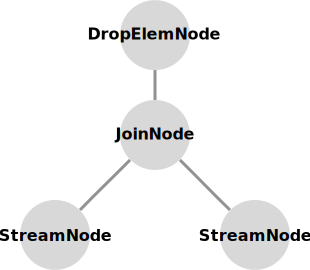
\includegraphics[scale=0.7]{images/graph.pdf}
\centering
\end{figure}

Some classes, e.g., \lstinline{JoinNode}, extend a trait called \lstinline{EsperEngine}, while others, e.g., \lstinline{FilterNode}, do not.
The actors extending \lstinline{EsperEngine} are essentially equipped with their own instance of the EP engine Esper \cite{esper}, which they use to perform the respective operation they represent.
This approach has two advantages.
At first, by relying on Esper's implementation of more complex operators, e.g., \lstinline{join}, a (possibly incorrect) implementation of such operators does not have to be provided.
Moreover, resolving the semantic ambiguity of the \lstinline{sequence} as well as the \lstinline{and} operator is also taken care of by Esper's implementation.
It is to be noted that some of the code of the \lstinline{EsperEngine} trait was inspired by a Lightbend Activator Template called ``CEP with Akka and Esper or Streams'' \cite{akkacep}.

Obviously, the execution graph of a query is created dynamically at run-time.
At first, a \lstinline{Node} corresponding to the outermost query of the respective query is created as a top-level actor of an \lstinline{ActorSystem}.
From then on, the graph builds up recursively, i.e., a \lstinline{UnaryNode} will create a child actor that corresponds to the one subquery of the \lstinline{UnaryQuery} which it represents.
Likewise, a \lstinline{BinaryNode} will create two child actors that correspond to the two subqueries of the \lstinline{BinaryQuery} which it represents.
\lstinline{LeafNode}s will issue \lstinline{Subscription}(s) to \lstinline{Publisher}(s).
When a \lstinline{Publisher} acknowledges a \lstinline{LeafNode}'s subscription, the \lstinline{LeafNode} either sends a \lstinline{Created} message to its parent actor, or---if it is the root actor of the graph---invokes a closure that is to be called as soon as the graph is fully built (which supplied by the user). \lstinline{UnaryNode}s and \lstinline{BinaryNode}s also either send a \lstinline{Created} message to their parent actors or call the aforementioned closure as soon as all of their child actors have sent them the \lstinline{Created} message.

Finally, it is noteworthy that at run-time, events are represented by the classes \lstinline{Event1}, \lstinline{Event2}, ..., \lstinline{Event6}, all of which extend the trait \lstinline{Event}.
\lstinline{Publisher}s pass up \lstinline{Event}s to the leaves of an execution graph and, within this graph, \lstinline{Node}s pass them up to their parent actors.
Unlike their counterparts \lstinline{Query1}, \lstinline{Query2}, ..., \lstinline{Query6}, \lstinline{Event}s do not have type parameters for each of their elements.
Instead, the elements of an \lstinline{Event} are of type \lstinline{Any}.
However, Akka actors are untyped anyway, i.e., actors receive any message and can send any message to any actor.

\subsection{Quality of Service}
\label{sec:qos}

As the title of this thesis suggests, EventScala represents a QoS-oriented approach to EP.
As such, it allows not only for QoS requirements to be defined over queries but also for their enforcement at run-time.
To this end, the execution graph that EventScala's execution engine creates for a given query features so-called QoS monitors.
These surveil an actor's performance and carry out a user-defined reaction when a requirement is not met.

This section is structured as follows.
At first, the notion of QoS monitors is introduced conceptually.
Then, implementation details are laid out.
Lastly, the two exemplary monitors that come with EventScala are described.

Conceptually, when picturing a query as a graph, QoS requirements can be defined over each node of that graph.
To be more precise, an arbitrary amount of \lstinline{FrequencyRequirement}s and \lstinline{LatencyRequirement}s can be defined over each node of the graph.
As this conceptual graph precisely resembles the execution graph of the same query, QoS requirements of a (sub)query are being dealt with by the actor that represents the (sub)query in the execution graph.
Therefore, each actor has to monitor its performance, and, whenever a requirement is not being met, react to this circumstance by invoking a closure that has been specified along with the respective requirement.
(To this end, both case classes \lstinline{FrequencyRequirement} and \lstinline{LatencyRequirement} specify a field named \lstinline{callback}.)
This closure might even carry out curative measures, as its arguments include the respective actor's \lstinline{ActorContext}, which embodies run-time information about the actor.

Informally speaking, in order to create an execution graph for a given query, EventScala's execution engine requires the user to provide reference to one class representing a frequency monitor as well as to one class representing a latency monitor.
At run-time, each actor of the execution graph gets exactly one instance of both of them---regardless of whether or not the query that the actor represents specifies any QoS requirements.
As a consequence, at run-time, each actor has one frequency monitor instance as well as one latency monitor instance.

Technically speaking, EventScala's execution engine requires the user to provide two classes that extend the \lstinline{MonitorFactory} trait, one for frequency monitoring and one for latency monitoring.
A \lstinline{MonitorFactory} can create instances of classes that extend one of the traits \lstinline{LeafNodeMonitor}, \lstinline{UnaryNodeMonitor} or \lstinline{BinaryNodeMonitor}.
Thus, at run-time, a \lstinline{LeafNode} will have a \lstinline{LeafNodeMonitor} for frequency monitoring as well another \lstinline{LeafNodeMonitor} for latency monitoring.
The former will have been created by the factory supplied for frequency monitoring and the latter will have been created by the factory supplied for latency monitoring.
Analogously, the same is true for \lstinline{UnaryNode}s and \lstinline{BinaryNode}s.

EventScala has been designed to make it easy for users to implement their own monitors.
To do so, one has to provide four classes that implement the four traits \lstinline{LeafNodeMonitor}, \lstinline{UnaryNodeMonitor}, \lstinline{BinaryNodeMonitor} as well as \lstinline{MonitorFactory}, respectively.
EventScala comes with one exemplary frequency monitor as well as with one exemplary latency monitor. The examplary frequency monitor, for instance, is comprised of the following four classes:

\begin{itemize}
\item
\lstinline{AverageFrequencyLeafNodeMonitor} extending the trait \lstinline{LeafNodeMonitor}
\item
\lstinline{AverageFrequencyUnaryNodeMonitor} extending the trait \lstinline{UnaryNodeMonitor}
\item
\lstinline{AverageFrequencyBinaryNodeMonitor} extending the trait \lstinline{BinaryNodeMonitor}
\item
\lstinline{AverageFrequencyMonitorFactory} extending the trait \lstinline{MonitorFactory}
\end{itemize}

However, the question remains how these monitors actually surveil the performance of the actor they are associated with.
Each monitor implements so-called lifecycle methods, i.e., hooks into the respective actor's lifecycle.
This approach has been inspired by React, Facebook's JavaScript library for building UIs \cite{react}, in which so-called components have so-called lifecycle methods ``that you can override to run code at particular times in the process'' \cite{reactcomponent}.
\lstinline{LeafNodeMonitor}, \lstinline{UnaryNodeMonitor} and \lstinline{BinaryNodeMonitor} all specify three methods that need to be implemented by extending classes:

\begin{itemize}
\item
\lstinline{onCreated}
\item
\lstinline{onEventEmit}
\item
\lstinline{onMessageReceive}
\end{itemize}

As the names of these methods suggest, the actors of an execution graph invoke them at certain times during their lifecycle.
\lstinline{onCreated} is being called only once, right after all of the actor's children have issued a \lstinline{Created} message to it.
\lstinline{onEventEmit} is being invoked whenever the actor emits an event.
\lstinline{onMessageReceive} is being called whenever the actor receives a message that has not been generated by the execution graph, as it might have been sent by another monitor.
(This way, communication between the monitors of the actors of a graph is facilitated.)
Obviously, whenever \lstinline{onEventEmit} is called, it is passed the respective event as an argument.
Likewise, whenever \lstinline{onMessageReceive} is called, it is passed the respective message.
Furthermore, depending on the type of the respective actor, when being invoked, all three methods are always passed either an instance of the \lstinline{LeafNodeData} case class, an instance of the \lstinline{UnaryNodeData} case class or an instance of the \lstinline{BinaryNodeData} case class.
All of these contain the name of the respective actor as a \lstinline{String} as well as its \lstinline{ActorContext}.
\lstinline{UnaryNodeData} and \lstinline{BinaryNodeData} also contain an \lstinline{ActorRef}, i.e., a reference to an actor, for each of their child actors, i.e., child nodes.

To conclude, it should be noted that this approach constitutes a powerful way to surveil the performance of an actor and, by extension, the performance of the entire execution graph.
For each metric (frequency and latency), each actor has one monitor.
A monitor contains code that is being executed repeatedly throughout the lifecycle of an actor.
The methods embodying this code are invoked with run-time information about the actor.
Moreover, monitors are able to communicate with each other using messages.
As monitors are nothing but classes extending one of the traits \lstinline{LeafNodeMonitor}, \lstinline{UnaryNodeMonitor} or \lstinline{BinaryNodeMonitor}, they can leverage the capabilities of Scala classes, e.g., keeping state in field variables of the class.

As mentioned before, EventScala comes with one exemplary frequency monitor as well as one exemplary latency monitor.
The following two paragraphs will informally describe them.

The exemplary frequency monitor, called average frequency monitor, is comprised of four classes, which are all defined in one file \lstinline{AverageFrequencyMonitor.scala}.
When setting up EventScala's execution engine to use it for frequency monitoring, the user needs to supply an interval, e.g., 30 seconds.
The monitor instance of each actor of the resulting execution graph uses a field variable to keep track of the number of events emitted by that actor.
Whenever the interval is up, e.g., every 30 seconds, the monitor uses that number to calculate whether \lstinline{FrequencyRequirement}s have been met.
Then, it sets the counter back to zero.
For example, assume that a query that is represented by a monitor's actor contains the requirement \lstinline{frequency > ratio(2.instances, 5.seconds) /* ... */}.
If the actor emitted 12 events in the last 30 seconds, the monitor would calculate that---on \emph{average}---the actor emits 2 events in 5 seconds.
This would not satisfy the requirement, so the monitor would invoke the closure of the requirement.

The exemplary latency monitor, called path latency monitor, is also comprised of four classes, all of which are located in one file called \lstinline{PathLatencyMonitor.scala}.
This is a more complex monitor as it leverages communication between the monitor instances using messages.
Periodically, each monitor calculates the so-called path latency of its respective actor.
Given all paths that connect the actor in question to \lstinline{LeafNode}s, path latency denotes the time it takes a message, i.e., an event, to travel along the slowest of these paths.
Figure \ref{fig:latency} illustrates this concept by highlighting the path that is used to calculate the path latency of a node ``X''.
Obviously, the path latency of a \lstinline{LeafNode} is always 0.
In order to calculate it for \lstinline{UnaryNode}s and \lstinline{BinaryNode}s, each monitor surveiling such a node periodically sends a message to its child's or its children's monitor(s), respectively, which will respond immediately.
The time that passes between sending the message and receiving the response is being divided by 2 in order to approximate the time it takes for an event to travel from a child actor to the actor in question.
This value is referred to as child latency.
Obviously, child latency equals path latency if the child actor of the actor in question is a \lstinline{LeafNode}.
Path latency values are always advertised to the parent actor's monitor.
A \lstinline{UnaryNode}'s monitor can simply add the advertised path latency of its child actor to its child latency in order to obtain its own path latency.
A \lstinline{BinaryNode}'s monitor has to do so twice, i.e., it has to add the advertised path latency of child actor 1 to the child latency of child actor 1, and then do so again for child actor 2.
The greater of the two resulting values will be adopted as the \lstinline{BinaryNode}'s path latency.
If a \lstinline{LatencyRequirement} has been defined over the query that an actor represents, the requirement's closure will be invoked if the calculated path latency does not satisfy the requirement.
Figure \ref{fig:latency} illustrates how to calculate path latency:
Of the 3 paths that connect actor ``X'' to a \lstinline{LeafNode}, the one indicated by the thick, red edges is the slowest.
Therefore, it is used to calculate ``X''s path latency, which is 1 ms + 3 ms = 4 ms. When setting up EventScala's execution engine to use the path latency monitor for latency monitoring, an interval has to be provided, denoting how often path latency values are to be re-calculated, thus, denoting how often latency requirements are to be checked.

\begin{figure}
\caption{Path latency illustration}
\label{fig:latency}
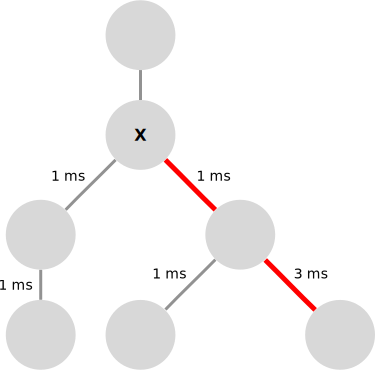
\includegraphics[scale=0.7]{images/latency.pdf}
\centering
\end{figure}

\newpage

\section{Simulation}
\label{sec:simulation}

In order to showcase its capabilities, EventScala comes with an exemplary set up simulating a real-world use case.
It is comprised of three main components:

\begin{itemize}
\item
4 sample \lstinline{Publisher}s representing four streams that can be subscribed to
\item
2 sample queries expressed using the DSL
\item
1 sample configuration for the execution engine
\end{itemize}

In this section, all three components are described in detail.
Then, the output that is being generated when running the simulation is discussed.

In EventScala, a publisher represents a primitive stream that can be subscribed to.
To this end, the specifications of the \lstinline{Publisher} trait (which, in turn, extends the \lstinline{Actor} trait) include that a publisher has to maintain a set of subscribers.
On top of that, EventScala defines a case class \lstinline{RandomPublisher}, which publishes one event every x milliseconds, with x being a pseudo-random \lstinline{Integer} between 0 (inclusive) and 5000 (exclusive).
A \lstinline{RandomPublisher} takes a closure of type \lstinline{Integer => Event}, which it invokes in order to obtain the \lstinline{Event} instances it publishes.
To obtain the first event, it calls the closure with \lstinline{0}, to invoke the second event, it calls the closure with \lstinline{1}, and so on.
In the simulation, there are four \lstinline{RandomPublisher}s called ``A'', ``B'', ``C'' and ``D'', representing streams of the types \lstinline{Stream1[Int]}, \lstinline{Stream1[Int]}, \lstinline{Stream1[Float]} and \lstinline{Stream1[String]}, respectively, as shown in listing \ref{lst:sim_publishers}.

\begin{lstlisting}[
caption={The four \lstinline{RandomPublisher}s of the simulation},
label={lst:sim_publishers}]
val publisherA: ActorRef = actorSystem.actorOf(Props(
  RandomPublisher(id => Event1(id))), "A")
val publisherB: ActorRef = actorSystem.actorOf(Props(
  RandomPublisher(id => Event1(id * 2))), "B")
val publisherC: ActorRef = actorSystem.actorOf(Props(
  RandomPublisher(id => Event1(id.toFloat))), "C")
val publisherD: ActorRef = actorSystem.actorOf(Props(
  RandomPublisher(id => Event1(s"String($id)"))), "D")
\end{lstlisting}

The two sample queries \lstinline{query1} and \lstinline{query2} (shown in listing \ref{lst:sim_queries}) are expressed using the DSL and should not require any further explanation.
\lstinline{query1} will not be presented below as it is the same query that is shown in listing \ref{lst:dsl_qos}.

\begin{lstlisting}[
caption={\lstinline{query2} of the simulation},
label={lst:sim_queries}]
val query2: Query4[Int, Int, Float, String] =
  stream[Int]("A")
  .and(stream[Int]("B"))
  .join(
    sequence(
      nStream[Float]("C") -> nStream[String]("D"),
      frequency > ratio(1.instances, 5.seconds) otherwise { (nodeData) =>
        println(s"PROBLEM:\tNode `${nodeData.name}` emits too few events!") }),
    slidingWindow(3.seconds),
    slidingWindow(3.seconds),
    latency < timespan(1.milliseconds) otherwise { (nodeData) =>
      println(s"PROBLEM:\tEvents reach node `${nodeData.name}` too slowly!") })
\end{lstlisting}

Lastly, the simulation comes with a sample configuration for the execution graph that EventScala's execution engine creates for either \lstinline{query1} and \lstinline{query2}.
(Shown in listing \ref{lst:sim_conf} is the version for \lstinline{query1}.)
It is specified that the exemplary monitors, i.e., \lstinline{AverageFrequencyMonitor} and \lstinline{PathLatencyMonitor}, will be used for frequency and latency monitoring, respectively.
The former is set to perform its calculations every 15 seconds while the latter is set to do so every 5 seconds.
Both of them are set to log their calculations to the console.
The closure that will be invoked when the graph has been created simply prints \lstinline{"STATUS:\tGraph has been created."} to the console, and the closure that will be called whenever the root actor produced an event simply prints said event to the console.
It is to be noted that the latter closure is type-safe, i.e., its type is \lstinline{Either[Int, String], Either[Int, X], Either[Float, X] => Any}.

\begin{lstlisting}[
caption={The execution graph configuration of the simulation (Newlines were added to fit the page.)},
label={lst:sim_conf}]
val graph: ActorRef = GraphFactory.create(
  actorSystem =             actorSystem,
  query =                   query1,
  publishers =              publishers,
  frequencyMonitorFactory = AverageFrequencyMonitorFactory 
                            (interval = 15, logging = true),
  latencyMonitorFactory =   PathLatencyMonitorFactory
                            (interval =  5, logging = true),
  createdCallback =         () => println("STATUS:\tGraph has been created."))(
  eventCallback =           {
    case (Left(i1), Left(i2), Left(f)) =>
      println(s"COMPLEX EVENT:\tEvent3($i1,$i2,$f)")
    case (Right(s), _, _) =>
      println(s"COMPLEX EVENT:\tEvent1($s)")
    // This is necessary to avoid warnings about non-exhaustive `match`:
    case _ =>
  })
\end{lstlisting}

When being run for approximately 15 seconds (not including set up time) on a Lenovo ThinkPad X220i laptop with a Intel Core i3-2350M CPU @ 2.30 GHz * 2 processor, this simulation generates the console output like shown in listing \ref{lst:sim_out}.

\begin{lstlisting}[
caption={The console output of the simulation (Newlines were added to fit the page.)},
label={lst:sim_out}]
STATUS:         Graph has been created.
LATENCY:
  Events reach node `disjunction-1-conjunction-1-selfjoin-1-dropelem` after
  PT0.015S. (Calculated every 5 seconds.)
PROBLEM:
  Events reach node `disjunction-1-conjunction-1-selfjoin-1-dropelem` too slowly!
STREAM A:       Event1(1)
STREAM B:       Event1(2)
STREAM A:       Event1(2)
STREAM D:       Event1(String(2))
COMPLEX EVENT:  Event1(String(2))
STREAM C:       Event1(1.0)
COMPLEX EVENT:  Event3(2,2,1.0)
STREAM B:       Event1(4)
STREAM A:       Event1(3)
STREAM C:       Event1(2.0)
COMPLEX EVENT:  Event3(4,4,2.0)
LATENCY:
  Events reach node `disjunction-1-conjunction-1-selfjoin-1-dropelem` after
  PT0.0015S. (Calculated every 5 seconds.)
PROBLEM:
  Events reach node `disjunction-1-conjunction-1-selfjoin-1-dropelem` too slowly!
STREAM D:       Event1(String(3))
COMPLEX EVENT:  Event1(String(3))
STREAM C:       Event1(3.0)
STREAM B:       Event1(6)
STREAM D:       Event1(String(4))
COMPLEX EVENT:  Event1(String(4))
STREAM C:       Event1(4.0)
STREAM B:       Event1(8)
STREAM A:       Event1(4)
COMPLEX EVENT:  Event3(8,8,3.0)
STREAM C:       Event1(5.0)
STREAM B:       Event1(10)
COMPLEX EVENT:  Event3(10,10,5.0)
STREAM D:       Event1(String(5))
COMPLEX EVENT:  Event1(String(5))
LATENCY:
  Events reach node `disjunction-1-conjunction-1-selfjoin-1-dropelem` after
  PT0.0005S. (Calculated every 5 seconds.)
STREAM C:       Event1(6.0)
STREAM A:       Event1(5)
COMPLEX EVENT:  Event3(10,10,6.0)
STREAM B:       Event1(12)
STREAM B:       Event1(14)
STREAM A:       Event1(6)
STREAM C:       Event1(7.0)
COMPLEX EVENT:  Event3(12,12,7.0)
STREAM C:       Event1(8.0)
STREAM D:       Event1(String(6))
COMPLEX EVENT:  Event1(String(6))
LATENCY:
  Events reach node `disjunction-1-conjunction-1-selfjoin-1-dropelem` after
  PT0.0015S. (Calculated every 5 seconds.)
PROBLEM:
  Events reach node `disjunction-1-conjunction-1-selfjoin-1-dropelem` too slowly!
FREQUENCY:
  On average, node `disjunction-1-conjunction-1-selfjoin` emits 3 events every
  5 seconds. (Calculated every 15 seconds.)
PROBLEM:
  Node `disjunction-1-conjunction-1-selfjoin` emits too few events!
FREQUENCY:
  On average, node `disjunction-1-conjunction-1-selfjoin` emits 9 events every
  15 seconds. (Calculated every 15 seconds.)
\end{lstlisting}

It can be observed that publishers print the primitive events they publish to the console.
Likewise, the root node prints the complex events the execution graph produces to the console.
As expected, the latency monitor of the node \lstinline{disjunction-1-conjunction-1-selfjoin-1-dropelem} logged to the console four times, i.e., once after graph creation, once after 5 seconds, once after 10 seconds, and once after 15 seconds.
Also as expected, the frequency monitor of the node \lstinline{disjunction-1-conjunction-1-selfjoin} only logged to the console once, i.e., after 15 seconds.
Lastly, it is to be noted that the latency requirement has been met in 1 out of 4 times.
The two frequency requirements, however, are defined in a way that they can never both be met.
Accordingly, after 15 seconds, one of them was met (\lstinline{frequency < ratio(12.instances, 15.seconds)}) while the other one was not (\lstinline{frequency > ratio(3.instances, 5.seconds)}).

\newpage

\section{Conclusion}
\label{sec:conclusion}

This thesis set out to explore ways to solve some of the existing problems of current EP solutions, i.e., the communication of queries in the form of strings (e.g., \cite{esper}), the absence of concurrent execution from industry-grade solutions \cite{Schilling:2010:DHE:1827418.1827453} and the missing ability to express QoS requirements as part of a query.
To this end, the EventScala framework has been proposed in this thesis, constituting a type-safe, distributed and QoS-oriented approach to EP.

It can be concluded that using EventScala's DSL to express queries is an approach superior to expressing them in the form of strings.
Errors in such strings cannot be detected at compile-time, therefore, they will cause failure at run-time.
To the contrary, queries expressed using the DSL are nothing but Scala expressions, thus, they are type-checked at compile-time.
Syntactic errors such as misspelled method names are caught during compilation just like type-related errors, e.g., the \lstinline{dropElem3} operator cannot be applied to a stream of events that consist of only two or less elements.

Furthermore, it can be stated that EventScala introduces a highly distributed approach to executing queries.
With each primitive and operator of a query being represented by a processing node, i.e., by an Akka actor, the benefits of concurrent execution can be reaped.
For example, parallel execution can be employed for performance gains, parts of the processing can be moved to be in proximity of publishers, etc.

Lastly, an approach to support the annotation of queries with QoS requirements at the language as well as the execution level has been presented.
The proposed DSL represents a way to incorporate such requirements on a per-query basis into a query language.
EventScala's execution engine constitutues a novel way to run a query while monitoring run-time performance and reacting to non-met requirements.

As the EventScala framework is the contribution of a bachelor thesis, it is merely a prototype, missing many of the features of industry-grade solutions. E.g., at the execution level, fault tolerance has not been considered. Nevertheless, as successfully demonstrated with the simulation, EventScala can be used to define and run non-trivial queries, featuring stream subscriptions from various publishers, operators from both SP and CEP as well as several QoS requirements.

\newpage

\printbibliography

\end{document}
